\section*{Appendix}
\vspace{.3in}

\section{Experimental Details}
\label{sec:exp-details}

Table~\ref{tab:operators} lists the attention operators and the models they are extracted from,
and Table~\ref{tab:baselines} lists the versions and configurations of all baselines.
Each baseline supports a subset of the setups we evaluate.

For throughput, following~\cite{Megatron-LM}, we calculate the theoretical
floating-point operations (FLOPs) required for the attention computation
based on the model configuration (such as sequence length, number of heads, and hidden
dimension) and divide it by the measured latency.
We measure end-to-end latency with the CUDA Events API,
and kernel latency in operator experiments with Nsight Systems (\texttt{nsys})
for better precision on short-duration kernels.

\begin{table}[h]
  \small
  \centering
  \caption{LLM operators used in our evaluation. }
  \label{tab:operators}
  \begin{tabular}{l|l|l} \Xhline{2\arrayrulewidth}
    \textbf{Operator} & \textbf{Description}    & \textbf{Base Arch.} \\ \hline
    Global      & Global Attention        & ViT 1.2B \\
    Causal      & Causal Attention (MHA)  & \makecell[l]{Llama 2 7B, Qwen2 7B, \\ Qwen3 8B} \\
    GQA         & Grouped Query Attention & GLM-4 9B \\
    % \NA{Sparse} & \NA{Deepseek Sparse Attention} & \NA{DeepSeek-V3.2} \\
    \Xhline{2\arrayrulewidth}
  \end{tabular}
\end{table}

\begin{table}[h]
  \small
  \centering
  \caption{Baselines used in our evaluation.}
  \label{tab:baselines}
  \begin{tabular}{llll}
    \toprule
    \textbf{Baseline} & \textbf{Version} & \textbf{Kind} & \textbf{Configuration} \\
    \midrule
    Tawa~\cite{tawa}                    & 3.3            & Tile compiler & Stock attention, FlashAttention-3 strategy \\
    TileLang~\cite{tilelang}            & 0.1.8          & Tile compiler & Stock attention, FlashAttention-3 strategy \\
    OpenAI Triton~\cite{openai-fused-attn} & Triton 3.6.0 & Tile compiler & OpenAI's fused attention \\
    Tri-Dao Triton~\cite{flash-attn-repo}  & Triton 3.6.0 & Tile compiler & Dao-AILab's Triton attention \\
    Helion                              & 0.3.1          & Compiler      & \\
    FlexAttn                            & PyTorch 2.11.0 & Compiler      & \texttt{compile(mode=`max-autotune', backend=`inductor')} \\
    TVM~\cite{tvm}                      & 0.18           & Compiler      & \\
    \midrule
    cuDNN                               & 9.11.0         & Library       & \\
    Tri-Dao~\cite{flash-attn-repo}      & 2.8.3          & Library       & Dao-AILab's CUTLASS implementation \\
    FlashInfer~\cite{flashinfer}        & 0.6.7          & Library       & \\
    ThunderKittens~\cite{thunderkittens} & --            & Library       & Obtained from the ThunderKittens authors \\
    PyTorch~\cite{pytorch}              & 2.11.0         & Library       & \texttt{compile(mode=`max-autotune', backend=`inductor')} \\
    \bottomrule
  \end{tabular}
\end{table}

\clearpage

\section{\NAME{} vs Vendor Libraries}
\label{sec:vendor-libs}

Appendix~\ref{sec:vendor-libs} provides the full comparison of Nautilus against
heavily optimized vendor libraries on GH200 and RTX 5090,
including detailed results for different attention variants and
sequence lengths.



\begin{figure*}[hb!]
  \centering
  % First Row: GH200 Baseline
  \begin{subfigure}[b]{0.95\textwidth}
    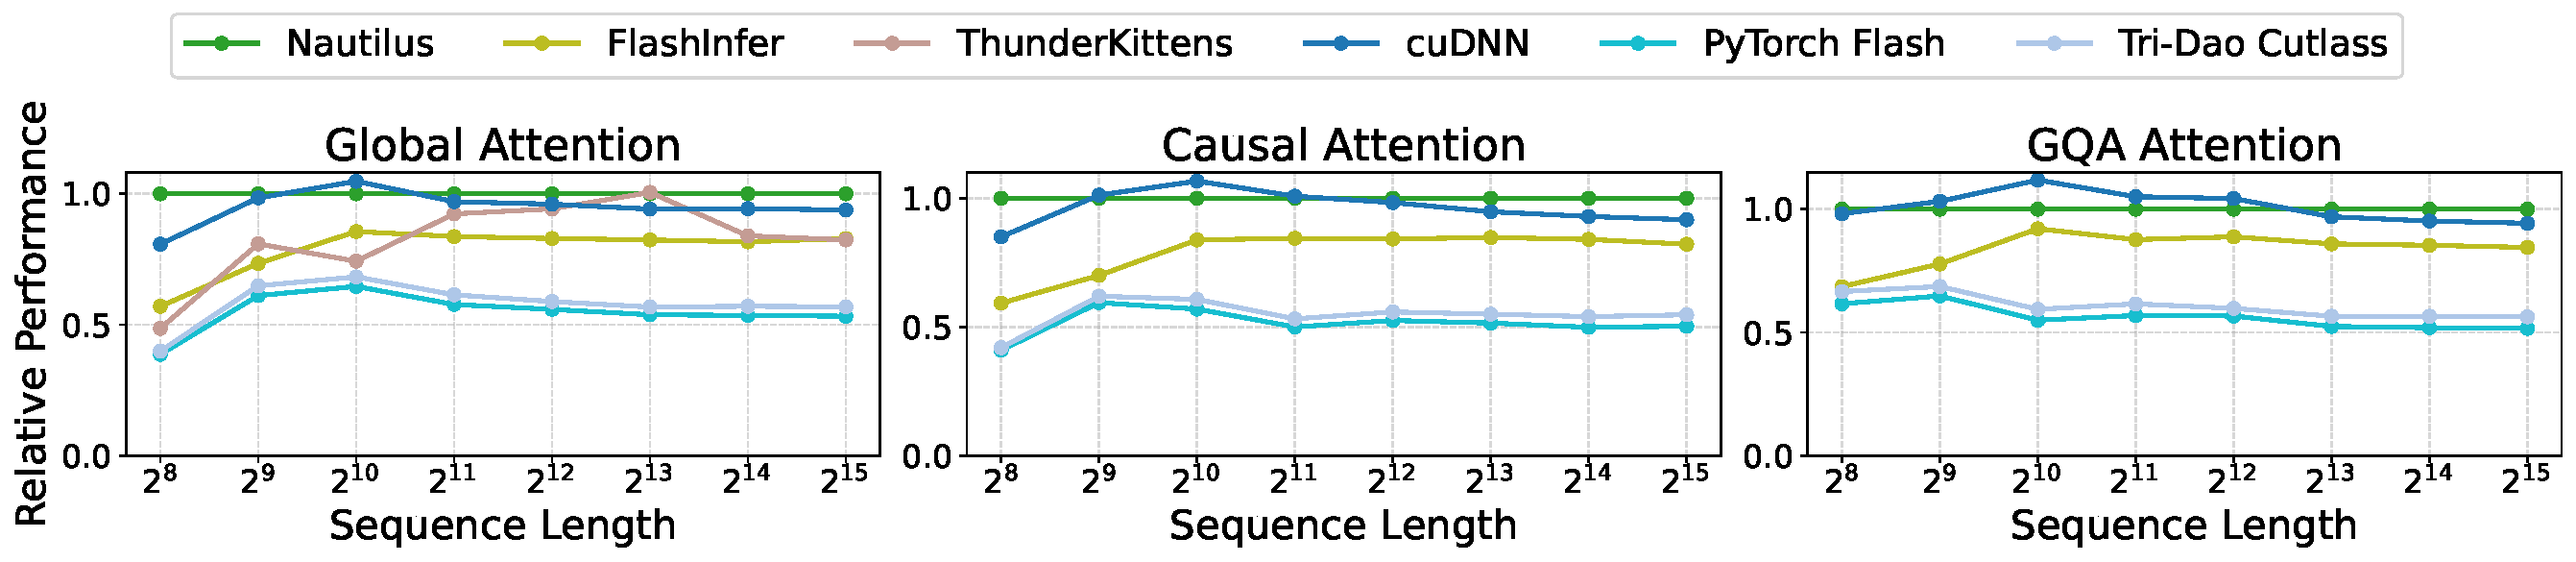
\includegraphics[width=\textwidth]{figures/gh200-fp16-baseline1.pdf}
    \vspace{-1.7em}
    \caption{GH200: FP16 performance (higher is better).}
    \label{fig:gh200-fp16-libs}
  \end{subfigure}

  % Second Row: RTX 5090 Baseline (New)
  \begin{subfigure}[b]{0.95\textwidth}
    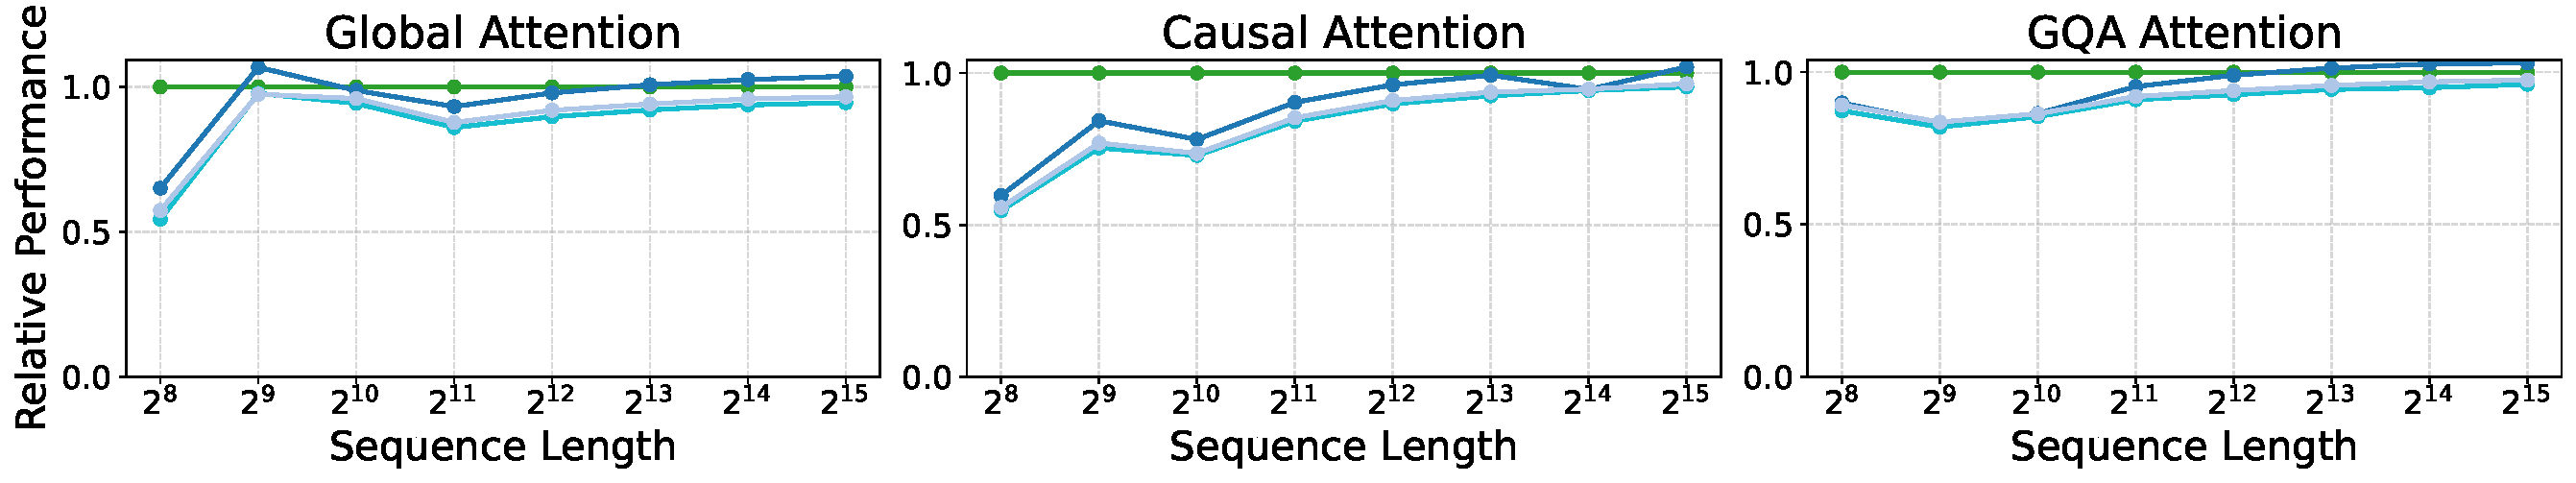
\includegraphics[width=\textwidth]{figures/rtx5090-fp16-baseline1.pdf}
    \vspace{-1.7em}
    \caption{RTX 5090: FP16 performance (higher is better).}
    \label{fig:rtx5090-fp16-libs}
  \end{subfigure}

  \caption{Performance of \NAME{} kernels vs. vendor libraries on GH200 and RTX 5090 platforms.
  The y-axis shows relative performance normalized to \NAME{} for each setup.}
  \label{fig:libs-prefill-comparison}
  %\vspace{-.15in}
\end{figure*}

\clearpage



\section{Numerical Stability of \NAME{} Kernels}
\label{sec:num-stab}

\noindent
\begin{minipage}[t]{0.46\textwidth}
\vspace{0pt}
Rewriting or re-associating floating-point operations can affect a kernel's numerical
behavior. To study this effect, we compare \NAME{}, Tri-Dao, and FlexAttention on
different attention operators. The results show that \NAME{} has competitive numerical
behavior. For all three systems, we use a common set of inputs and compare their outputs
to an FP64 unfused attention kernel baseline.
We keep the schedule and configuration of each kernel the same as in the performance
evaluation. To collect realistic attention inputs, we run a pretrained Qwen2.5 model
on 1000 WikiText sentences with sequence length 2048, and record the resulting input tensors.

In Table~\ref{tab:numeric_error_absolute_error}, we report the numerical error of the
three frameworks using root mean square error (RMS) together with the 90th and 99th
percentile error magnitudes. We also examine how per-sample (per-sentence) RMSE is
distributed. The results for PF Global, PF Causal, and PF GQA are shown in
Figure~\ref{fig:rmse-kde-all}. Overall, Nautilus stays very close to Tri-Dao
Attention in error and is consistently better than FlexAttention.
\end{minipage}%
\hfill
\begin{minipage}[t]{0.5\textwidth}
\vspace{0pt}
\centering\footnotesize\setlength{\tabcolsep}{4pt}

\captionof{table}{Numerical Error Summary for FP16 (Absolute Error)}
\label{tab:numeric_error_absolute_error}
\begin{tabular}{llrrr}
\hline
Method & Variant & RMS & 90th \% & 99th \% \\
\hline
\multirow{3}{*}{Nautilus}
& PF Global & 4.9e-05 & 5.1e-05 & 5.5e-05 \\
& PF Causal & 5.0e-05 & 5.1e-05 & 5.3e-05 \\
& PF GQA    & 5.0e-05 & 5.1e-05 & 5.3e-05 \\
\hline
\multirow{3}{*}{Tri-Dao Attention}
& PF Global & 4.8e-05 & 5.0e-05 & 5.1e-05 \\
& PF Causal & 4.9e-05 & 5.0e-05 & 5.2e-05 \\
& PF GQA    & 4.9e-05 & 5.0e-05 & 5.2e-05 \\
\hline
\multirow{3}{*}{Flex Attention}
& PF Global & 5.0e-05 & 5.2e-05 & 5.4e-05 \\
& PF Causal & 5.0e-05 & 5.1e-05 & 5.3e-05 \\
& PF GQA    & 5.0e-05 & 5.1e-05 & 5.3e-05 \\
\hline
\end{tabular}

\vspace{1em}
\captionof{table}{Numerical Error Summary for BF16 (Absolute Error)}
\label{tab:numeric_error_absolute_error_bf16}
\begin{tabular}{llrrr}
\hline
Method & Variant & RMS & 90th \% & 99th \% \\
\hline
\multirow{3}{*}{Nautilus}
& PF Global & 4.42e-04 & 4.45e-04 & 4.49e-04 \\
& PF Causal & 3.84e-04 & 3.87e-04 & 3.91e-04 \\
& PF GQA    & 3.83e-04 & 3.87e-04 & 3.90e-04 \\
\hline
\multirow{3}{*}{Tri-Dao Attention}
& PF Global & 4.41e-04 & 4.45e-04 & 4.48e-04 \\
& PF Causal & 3.84e-04 & 3.87e-04 & 3.91e-04 \\
& PF GQA    & 3.84e-04 & 3.87e-04 & 3.91e-04 \\
\hline
\multirow{3}{*}{Flex Attention}
& PF Global & 4.42e-04 & 4.45e-04 & 4.49e-04 \\
& PF Causal & 3.84e-04 & 3.87e-04 & 3.91e-04 \\
& PF GQA    & 3.84e-04 & 3.87e-04 & 3.91e-04 \\
\hline
\multirow{3}{*}{Flashlight}
& PF Global & 4.42e-04 & 4.45e-04 & 4.49e-04 \\
& PF Causal & 3.84e-04 & 3.87e-04 & 3.91e-04 \\
& PF GQA    & 3.84e-04 & 3.87e-04 & 3.91e-04 \\
\hline
\end{tabular}

\vspace{1em}
\captionof{table}{Numerical Error Summary for FP8 (Absolute Error)}
\label{tab:numeric_error_absolute_error_fp8}
\begin{tabular}{llrrr}
\hline
Method & Variant & RMS & 90th \% & 99th \% \\
\hline
\multirow{3}{*}{Nautilus}
& PF Global & 1.11e-02 & 1.28e-02 & 1.46e-02 \\
& PF Causal & 9.89e-03 & 1.12e-02 & 1.34e-02 \\
& PF GQA    & 9.88e-03 & 1.12e-02 & 1.34e-02 \\
\hline
\multirow{3}{*}{Tri-Dao Attention}
& PF Global & 1.16e-02 & 1.33e-02 & 1.50e-02 \\
& PF Causal & 1.02e-02 & 1.15e-02 & 1.37e-02 \\
& PF GQA    & 1.03e-02 & 1.16e-02 & 1.38e-02 \\
\hline
\multirow{3}{*}{Flex Attention}
& PF Global & 1.55e-02 & 1.68e-02 & 1.85e-02 \\
& PF Causal & 1.39e-02 & 1.50e-02 & 1.67e-02 \\
& PF GQA    & 1.39e-02 & 1.50e-02 & 1.67e-02 \\
\hline
\end{tabular}
\end{minipage}

\begin{figure}[h]
  \centering
\vspace{.2in}
  \begin{subfigure}[t]{0.32\textwidth}
    \centering
    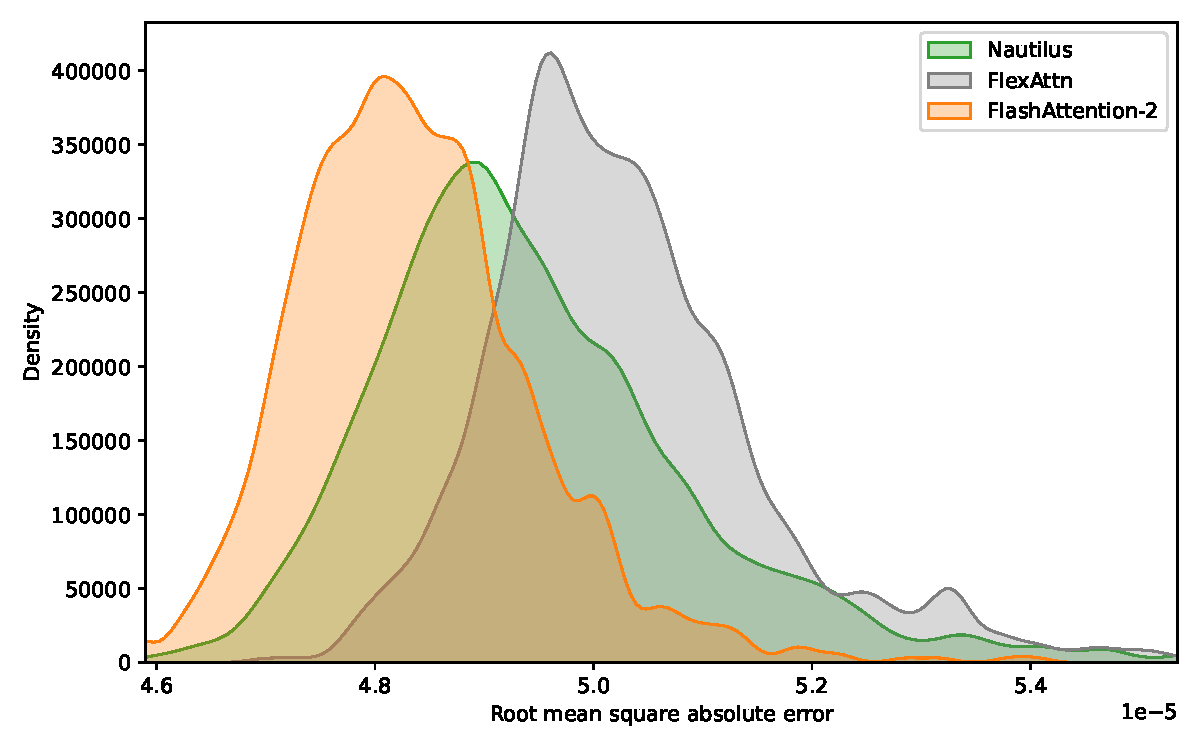
\includegraphics[width=\linewidth]{figures/qwen_rmse_kde_3curves_1000_global.pdf}
    \caption{PF Global.}
    \label{fig:rmse-kde-global}
  \end{subfigure}
  \hfill
  \begin{subfigure}[t]{0.32\textwidth}
    \centering
    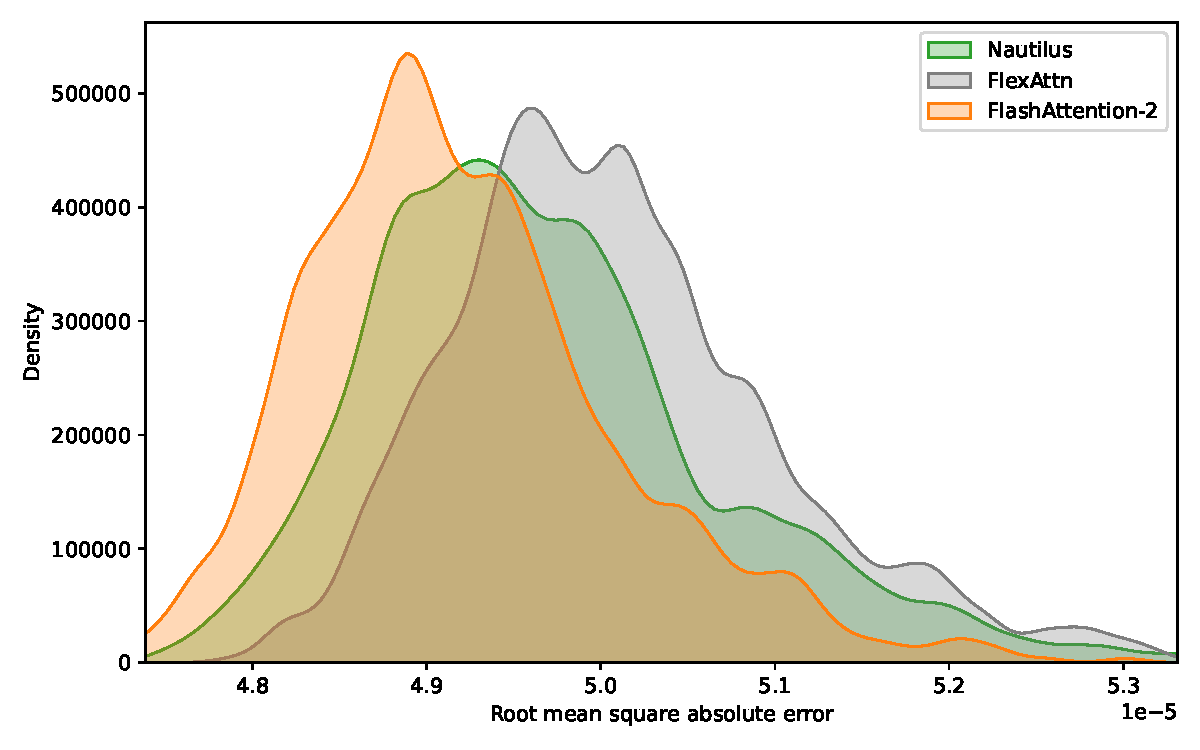
\includegraphics[width=\linewidth]{figures/qwen_rmse_kde_3curves_1000_causal.pdf}
    \caption{PF Causal.}
    \label{fig:rmse-kde-causal}
  \end{subfigure}
  \hfill
  \begin{subfigure}[t]{0.32\textwidth}
    \centering
    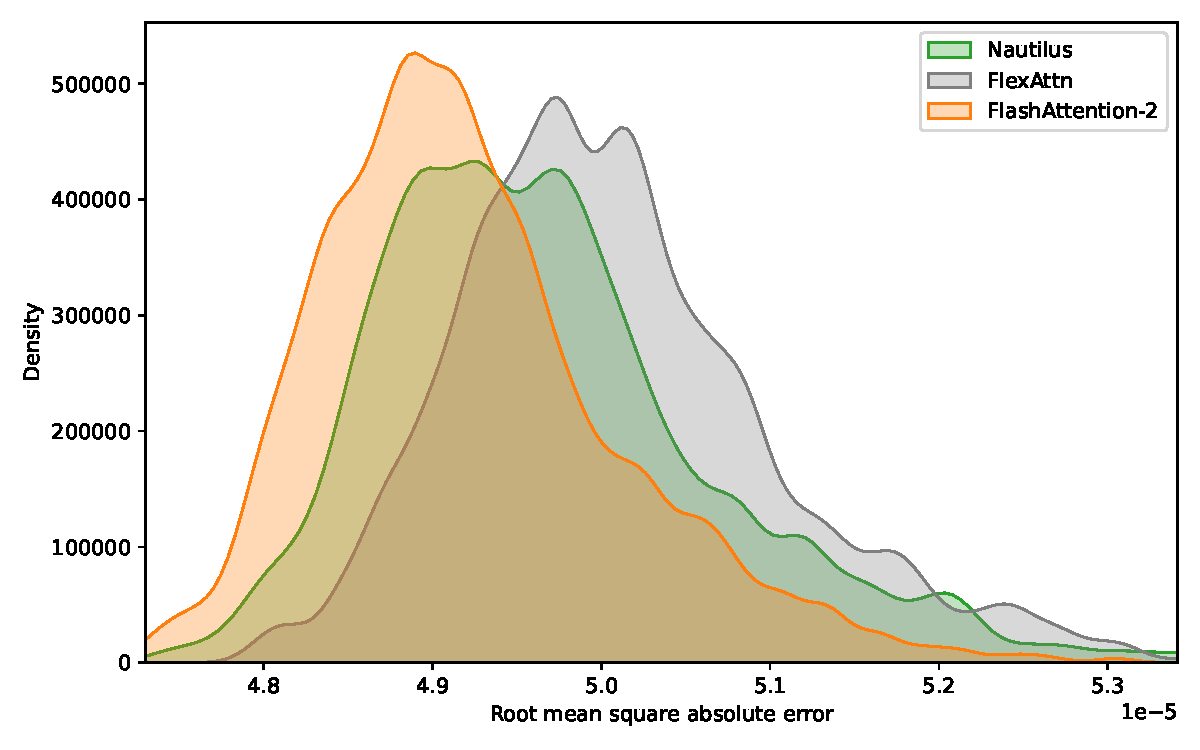
\includegraphics[width=\linewidth]{figures/qwen_rmse_kde_3curves_1000_gqa.pdf}
    \caption{PF GQA.}
    \label{fig:rmse-kde-gqa}
  \end{subfigure}

  \caption{Kernel numerical stability comparison on Qwen across three attention settings for FP16.}
  \label{fig:rmse-kde-all}
\end{figure}

\begin{figure}[h]
  \centering
\vspace{.2in}
  \begin{subfigure}[t]{0.32\textwidth}
    \centering
    \includegraphics[width=\linewidth]{figures/bf16_prefill_global_rmse.pdf}
    \caption{PF Global.}
    \label{fig:rmse-kde-global}
  \end{subfigure}
  \hfill
  \begin{subfigure}[t]{0.32\textwidth}
    \centering
    \includegraphics[width=\linewidth]{figures/bf16_prefill_causal_rmse.pdf}
    \caption{PF Causal.}
    \label{fig:rmse-kde-causal}
  \end{subfigure}
  \hfill
  \begin{subfigure}[t]{0.32\textwidth}
    \centering
    \includegraphics[width=\linewidth]{figures/bf16_prefill_gqa_rmse.pdf}
    \caption{PF GQA.}
    \label{fig:rmse-kde-gqa}
  \end{subfigure}

  \caption{Kernel numerical stability comparison on Qwen across three attention settings for BF16.}
  \label{fig:rmse-kde-all_bf16}
\end{figure}

\begin{figure}[h]
  \centering
\vspace{.2in}
  \begin{subfigure}[t]{0.32\textwidth}
    \centering
    \includegraphics[width=\linewidth]{figures/fp8_prefill_global_rmse.pdf}
    \caption{PF Global.}
    \label{fig:rmse-kde-global}
  \end{subfigure}
  \hfill
  \begin{subfigure}[t]{0.32\textwidth}
    \centering
    \includegraphics[width=\linewidth]{figures/fp8_prefill_causal_rmse.pdf}
    \caption{PF Causal.}
    \label{fig:rmse-kde-causal}
  \end{subfigure}
  \hfill
  \begin{subfigure}[t]{0.32\textwidth}
    \centering
    \includegraphics[width=\linewidth]{figures/fp8_prefill_gqa_rmse.pdf}
    \caption{PF GQA.}
    \label{fig:rmse-kde-gqa}
  \end{subfigure}

  \caption{Kernel numerical stability comparison on Qwen across three attention settings for FP8.}
  \label{fig:rmse-kde-all_bf16}
\end{figure}


\begin{table*}[t]
\centering
\small
\caption{Scheduling primitives used by the Nautilus auto-scheduler.}
\label{tab:primitives}
\begin{tabular}{clll}
\hline
Abbr. & Primitive & Short Description & Source \\
\hline
TL  & TileLoop($l_i$, $s_i$) & Split each $l_i$ into two loops with split factor $s_i$, and reorder these loops & TVM \\
BBI & BindBlockIdx($l$, \texttt{blockIdx}) & Fuse loops $l$ and associate them with a GPU thread block dimension & TVM \\
\hline
CRW & CacheReadWrite($n$, $t$, \texttt{place}) & Copy regions of $t$ accessed by $n$ from its current placement to \texttt{place} & TVM \\
SP  & SetPlacement($t$, \texttt{place}) & Set the placement of $t$ to \texttt{place}, affecting all accesses to $t$ & TVM \\
\hline
CI  & ComputeInline($n$, \texttt{dir}) & \begin{tabular}[c]{@{}l@{}}Inline the computation in $n$ into all producers/consumers,\\ and remove $n$ from the block graph\end{tabular} & TVM \\
CA  & ComputeAt($n$, $l$, \texttt{dir}) & Loop transformation-based operator fusion: fuse $n$ under $l$ & TVM \\
RU  & RollingUpdate($n_r$, $l$) & Advanced reduction operator fusion: fuse reduction $n_r$ under $l$ & Neptune \\
SKU & SplitKUpdate($n_r$, $l$) & \begin{tabular}[c]{@{}l@{}}Split reduction $n_r$ into local and global reductions,\\ and fuse the local reduction under $l$\end{tabular} & Neptune \\
\hline
DR  & DecomposeReduction($n_r$, $l$) & Move the initialization of reduction $n_r$ outside of $l$ & TVM \\
SSB & SplitScanBuffer($n_s$, $l$) & \begin{tabular}[c]{@{}l@{}}Multi-buffer the output of scan operation $n_s$\\ and update the buffers per $l$ iteration\end{tabular} & Neptune \\
\hline
PA  & PadAxis($n$, $t$, $a$, $e$) & \begin{tabular}[c]{@{}l@{}}Pad axis $a$ of $t$ to extent $e$ through every statement that carries it,\\ zero-filling inputs and cropping outputs\end{tabular} & Nautilus \\
PIE & PropagateIfThenElse($n$, $l$) & Narrow $l$ to the iterations where the mask in $n$ can hold & Neptune \\
FA  & FoldAccumulators($n$) & \begin{tabular}[c]{@{}l@{}}Fold terms added to a matmul in $n$ (bias, mask, other matmuls)\\ into its accumulator's initial value\end{tabular} & Nautilus \\
RB  & ReorderBlocks($l$, $o$) & Reorder the statements in the body of $l$ to legal order $o$ & Nautilus \\
\hline
\end{tabular}
\end{table*}



\begin{table*}[t]
\centering
\small
\caption{Tuning decisions in Nautilus schedules beyond the primitives' arguments. Structural choices fork
schedule seeds; sampled ones are recorded in the trace, so the auto-tuner mutates them and children
inherit good values.}
\label{tab:decisions}
\begin{tabular}{llll}
\hline
Decision & Values & Kind & Constraint / Note \\
\hline
Fusion strategy per reduction & classic, RU, SKU, RU+SKU hybrid & structural & \begin{tabular}[c]{@{}l@{}}Hybrid (3-level split) needs $\geq$16 rows in the tile\end{tabular} \\
Row padding                   & padded to 16, unpadded          & structural & Only for matmuls with $<$16 query rows (decode, MTP) \\
Tile loop sizes               & $s_i \in [32, 256]$             & sampled    & \begin{tabular}[c]{@{}l@{}}Accumulator side $\leq$128 and $M\!\times\!N \leq$ 1/4 of the register file;\\ reduction left whole if its operands fit half of shared memory\end{tabular} \\
Split count (hybrid)          & $[2,\ \mathrm{KV\ tiles}/2]$       & sampled    & Number of thread blocks splitting the KV axis \\
Warps per block               & 2, 4, 8                         & sampled    & Shared by all backends \\
Pipeline stages               & 0, 1, 2 (TileLang); 1, 2, 3 (Triton/Tawa) & sampled & \begin{tabular}[c]{@{}l@{}}On the rolling-update loop; lowered until the\\ multi-buffered tiles fit in shared memory\end{tabular} \\
Warp specialization           & off, on                         & sampled    & TileLang, sm\_90 and later \\
TMA copies                    & off, on                         & sampled    & TileLang, sm\_90 and later \\
Accumulator folding (FA)      & off, on                         & sampled    & Faster at small warp counts only \\
Statement order (RB)          & any legal order                 & sampled    & Uniform over orders keeping RAW/WAR/WAW dependencies \\
\hline
\end{tabular}
\end{table*}